\section{Pr\'esentation de Apache Griffin}


\subsection{Aperçu de l'outil}
Apache Griffin, est une solution open source de qualit\'e des donn\'ees pour le \textit{big data}. Il est d\'ecrit par ses concepteurs comme \'etant une plateforme offrant des services de qualit\'e des donn\'ees. De ce fait, il fournit un cadre complet d'analyse, permettant de r\'ealiser diverses t\^aches telles que la d\'efinition d'un mod\`ele de qualit\'e des donn\'ees, le calcul de diverses m\'etriques, l'automatisation de la validation des donn\'ees ainsi qu'une visualisation unifiée des m\'etriques. Gr\^ace aux infrastructures composant son \'ecosyst\`eme, Apache Griffin (Griffin) permet de g\'erer des donn\'ees venant aussi bien en temps r\'eel (\textit{streaming}) que par lot (\textit{batch}), tout en relevant les d\'efis en mati\`ere de qualit\'e dans les applications \textit{big data}. Face \`a l'absence de consensus sur la qualit\'e, Apache Griffin propose un standard sans pour autant \^etre restrictif.
\\

Conçu dans les locaux d'eBay en Mars 2016, puis confi\'e \`a la fondation Apache le 7 D\'ecembre de la m\^eme ann\'ee, Apache Griffin venait combler un certain nombre de besoins notamment \cite{ApacheGriffinIntro} : 
\begin{itemize}[parsep=0cm,itemsep=0cm]
\item le suivi de la qualit\'e  depuis de multiples sources de donn\'ees jusqu'aux applications cibles, tout en tenant compte de leurs historiques;

\item l'\'evaluation de la qualit\'e des donn\'ees en \textit{streaming} et en \textit{batch} tout en offrant la possibilit\'e de suivre l'évolution des diff\'erentes m\'etriques;

\item la mise en place d'une plateforme exposant une \acrshort{api}, permettant aux développeurs d'impl\'ementer leur propre interface utilisateur.
\end{itemize}

\subsection{Fonctionnalit\'es  d'Apache Griffin}

Afin de satisfaire ces diff\'erents besoins, Apache Griffin propose de nombreuses fonctionnalit\'es. Telles que pr\'esent\'ees dans la documentation, nous avons: 

\begin{itemize}[parsep=0cm,itemsep=0cm]

\item \textbf{la d\'efinition de mesures} : l'exactitude, l'exhaustivité ou la compl\'etude, l'actualité, l'unicité, la validité, la cohérence; il s'agit des diff\'erentes dimensions de la qualit\'e des donn\'ees qui peuvent \^etre \'evalu\'ees. L’utilisateur peut créer, modifier, supprimer et planifier des jobs pour les données venant par batch ;

\item \textbf{la surveillance des anomalies} : l'\'etablissement d'attentes sp\'ecifiques pour détecter les données anormales, tout en offrant la possibilit\'e de les téléchargés  ;

\item \textbf{les alertes en cas de d\'etection d'anomalies} : signaler les problèmes de qualité des données par e-mail ou sur la plateforme;

\item \textbf{la surveillance visuelle} : gr\^ace \`a son interface web, on peut appr\'ecier l'\'etat de la qualité des données au fil du temps;

\item \textbf{le temps réel} : l'inspection de la qualité des données peut être effectuée en temps réel;

\item \textbf{l'\'elasticit\'e et l'agilit\'e} : gr\^ace \`a ses facult\'es, Griffin peut être utilisé pour l'analyse des données provenant de plusieurs entrepôts de données. De plus, il fonctionne dans un environnement (Spark et Hadoop) pouvant g\'erer de grands volumes de donn\'ees (1,2 Petaoctet soit 1000 T\'eraoctet, cas d'eBay);

\item \textbf{la simplicit\'e} : Griffin fournit une interface utilisateur simple et facile à utiliser qui peut gérer les données et les règles de qualité; en même temps, les utilisateurs peuvent visualiser les résultats de qualité des données et personnaliser le contenu de l'affichage par le biais du panneau de contrôle.

\end{itemize}

\begin{figure}[H]
  \caption{Fonctionnalit\'es de Apache Griffin}  \label{fig:xray}
  \begin{center}
    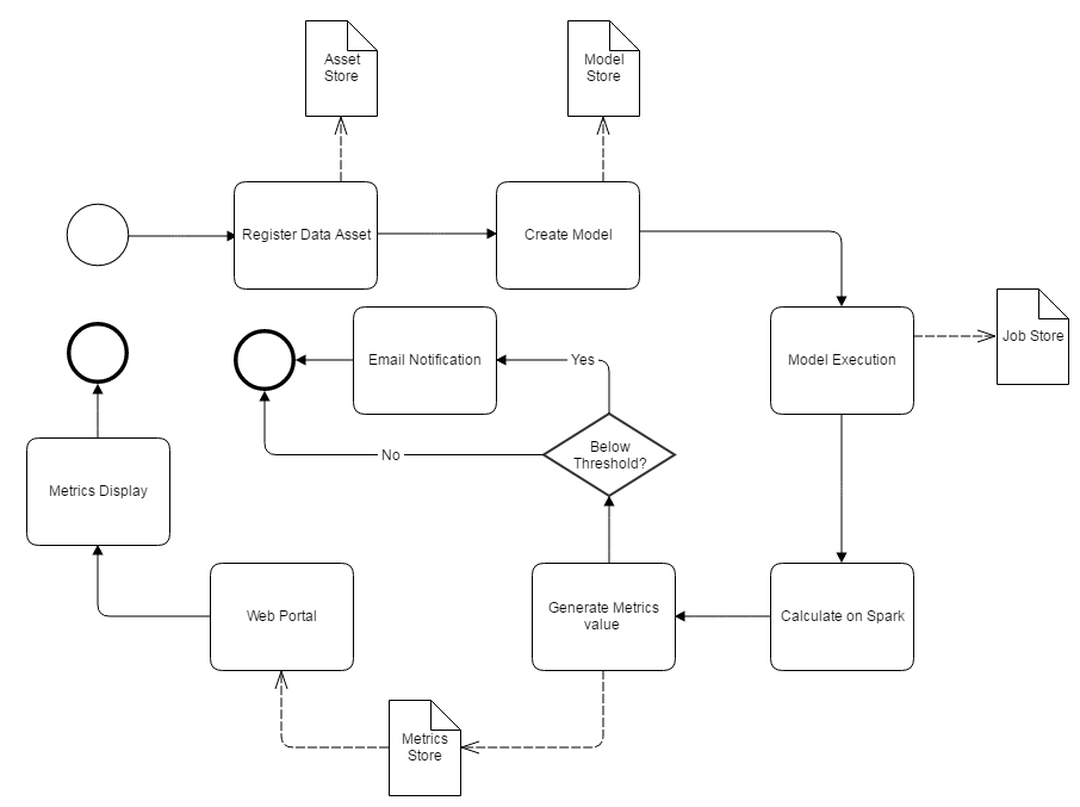
\includegraphics[scale=0.45]{Static/Capture.png} 
  \end{center}
\end{figure}

\subsection{Dimensions de la qualit\'e de donn\'ees}
 Dans cette sous-section, nous mettrons l'accent sur les langages de qualit\'e des donn\'ees de Griffin et sur les dimensions impl\'ement\'ees. En effet, les règles de qualit\'e des donn\'ees de Griffin sont \'edit\'ees soit \`a l'aide de  \emph{griffin-dsl} ou du \emph{spark-sql}. Tous deux ont pour syntaxe de base le \acrshort{sql}. Le \emph{griffin-dsl} est une surcouche du \emph{spark-sql}, mais moins verbeuse que ce dernier. Il suffit de pr\'eciser quelques mots cl\'es en fonction de la dimension choisie pour \'etablir la r\`egle voulue. Elle est ensuite traduite en \emph{spark-sql} puis ex\'ecut\'ee sur Apache Spark. Le \emph{spark-sql} est issu du module Spark \acrshort{sql} d'Apache Spark permettant de travailler avec des données structurées. Il permet de faire des requ\^etes sur Spark mais en utilisant le langage \acrshort{sql}, et cela peu importe la structure des donn\'ees. \\

Griffin offre \'egalement un certain formalisme en termes de qualit\'e des donn\'ees, dans la mesure o\`u il impl\'emente déjà en son sein plusieurs dimensions. Elles sont d\'efinies pour l'utilisation de \emph{griffin-dsl}. Au nombre de ces dimensions nous avons : 

\begin{description}[parsep=0cm,itemsep=0cm]
\item[Accuracy] : on cherche \`a obtenir le nombre de correspondances entre une donn\'ee source et une donn\'ee cible, conform\'ement \`a la dimension Exactitude. La d\'efinition de la règle décrit la relation de mappage entre les deux sources de données. Par exemple on a : "source.id = target.id and source.name = target.name";
\item[Profiling] : cette dimension permet de faire un profilage des donn\'ees. L'\'ecriture de la r\`egle peut se faire au moyen du langage \acrshort{sql} (\emph{spark-sql}) ou en \'ecriture simplifi\'ee (\emph{griffin-dsl}) comme: "source.id.count(), source.age.max() group by source.country";
\item[Distinctness] : il s'agit d'identifier les données qui sont en double (dimension Unicité). Pour ce faire, il suffit de pr\'eciser la ou les colonne(s) cibl\'ees s\'epar\'ees d'une virgule: "name, age";
\item[Completeness] : on vérifie ici si les valeurs d'une ou plusieurs colonnes sont nulles (dimension Exhaustivité). La r\`egle s'\'ecrit juste en pr\'ecisant la ou les colonnes dont on veut \'evaluer la compl\'etude;
\item[Timeliness] :  cette impl\'ementation mesure la latence de chaque élément et donne des statistiques de latence. Elle est disponible uniquement pour les donn\'ees en \textit{streaming}.
\end{description}
L'usage de \emph{spark-sql} peut \^etre vu comme un mode expert ou avanc\'e. Toutefois, la version 0.6.0 d'Apache Griffin n'offre que l'impl\'ementation de l'Accuracy, du Profiling et de la Completeness pour le \emph{griffin-dsl}. Pour l'impl\'ementation de nos r\`egles de qualit\'e nous avons fait une combinaison de \emph{spark-sql} et de \emph{griffin-dsl}.

\subsection{Architecture d'Apache Griffin}
\subsubsection{\textbf{Modules}}
L'outil est constitu\'e de trois (3) principaux modules : UI, Service, Measure. Le module UI pour \textit{User Interface}, est d\'evelopp\'e avec le \textit{framework} javascript Angular JS. Il s'agit du module qui g\`ere l'interface graphique de Apache Griffin. Il permet la visualisation des m\'etriques, leurs d\'efinitions et ordonnancement. Tout ceci est possible gr\^ace aux communications avec l'\acrshort{api} Service via le protocole \acrfull{http}. 
 %\begin{figure}[h]
 %   \begin{center}
 %     
\includegraphics[scale=0.65]{Static/create measure.png} 
%	\end{center}
%	\caption{Cr\'eation d'une mesure sur l'UI de Apache Griffin}  \label{fig:xray}
 %\end{figure}
 
\begin{figure}[H]
    \caption{UI de Apache Griffin} \label{fig:xray}
    \begin{center}
      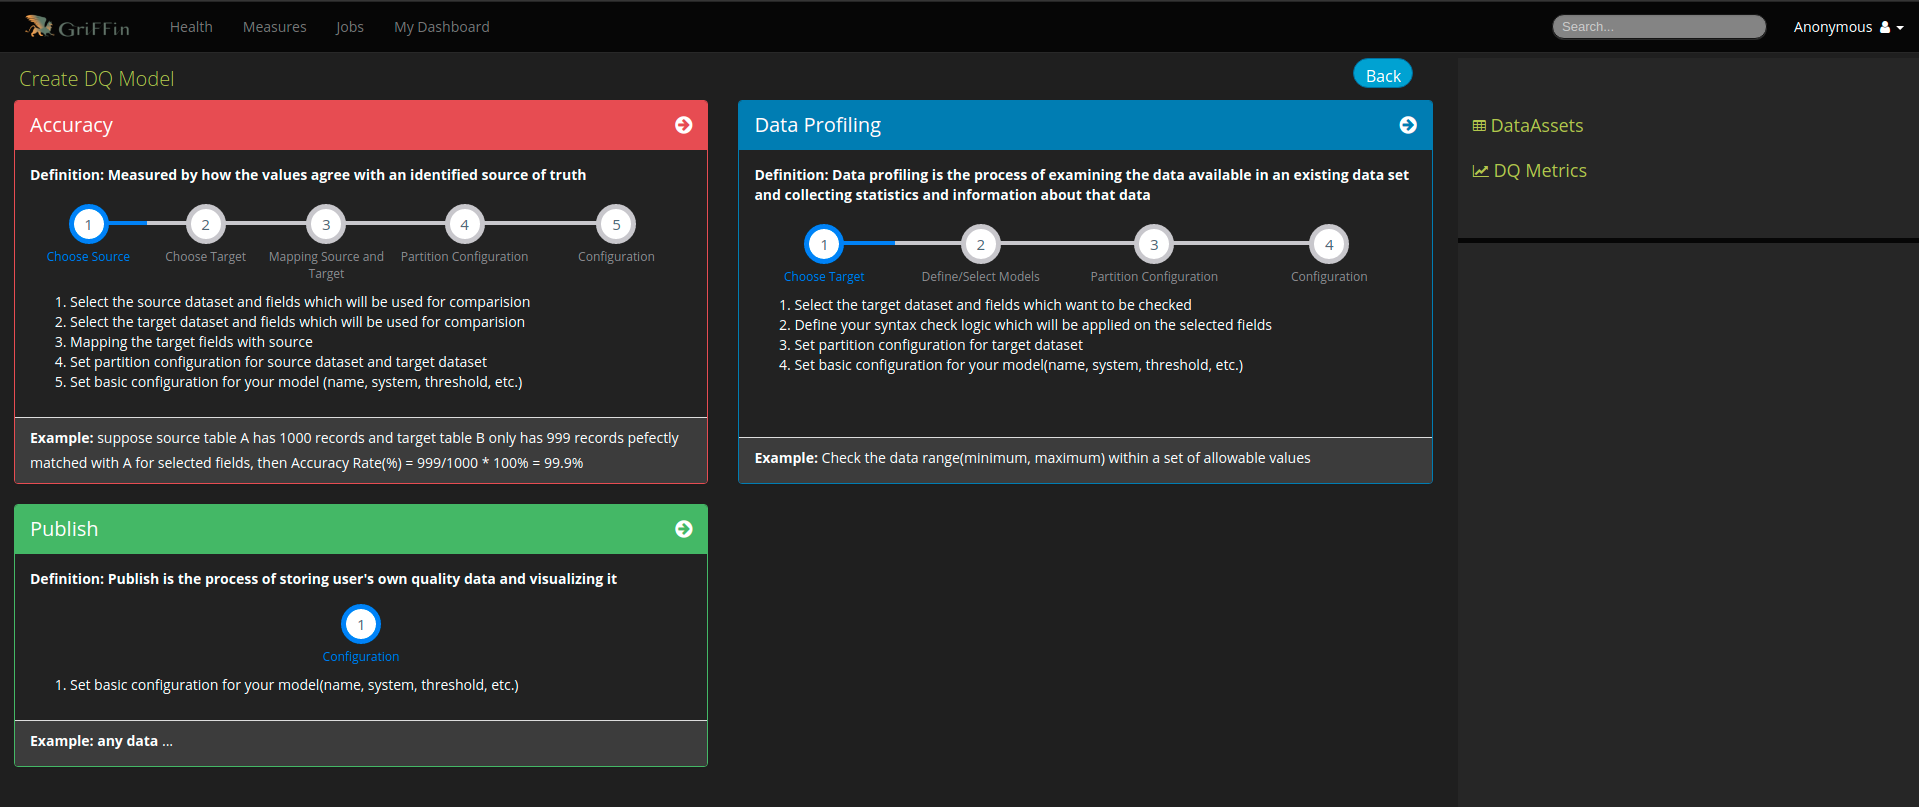
\includegraphics[scale=0.25]{Main/Static/UI_griffin.png} 
     \end{center}
\end{figure}
Le module Service, repr\'esente donc le web service de Apache Griffin. Développé en Java avec le \textit{framework} Spring Boot, il expose une \acrshort{api} \acrshort{rest}ful tr\`es riche. Elle offre bien plus de possibilit\'es qu'une utilisation via l'interface graphique, mais dans ce cas n\'ecessite de faire recours \`a un client tel que Postman pour les tests. Le calcul des diff\'erentes m\'etriques est fait par le module Measure, qui quant \`a lui est \'ecrit en Scala. 
\\
\begin{figure}[H]
    \caption{Interroger Apache Griffin avec Postman} \label{fig:xray}
    \begin{center}
      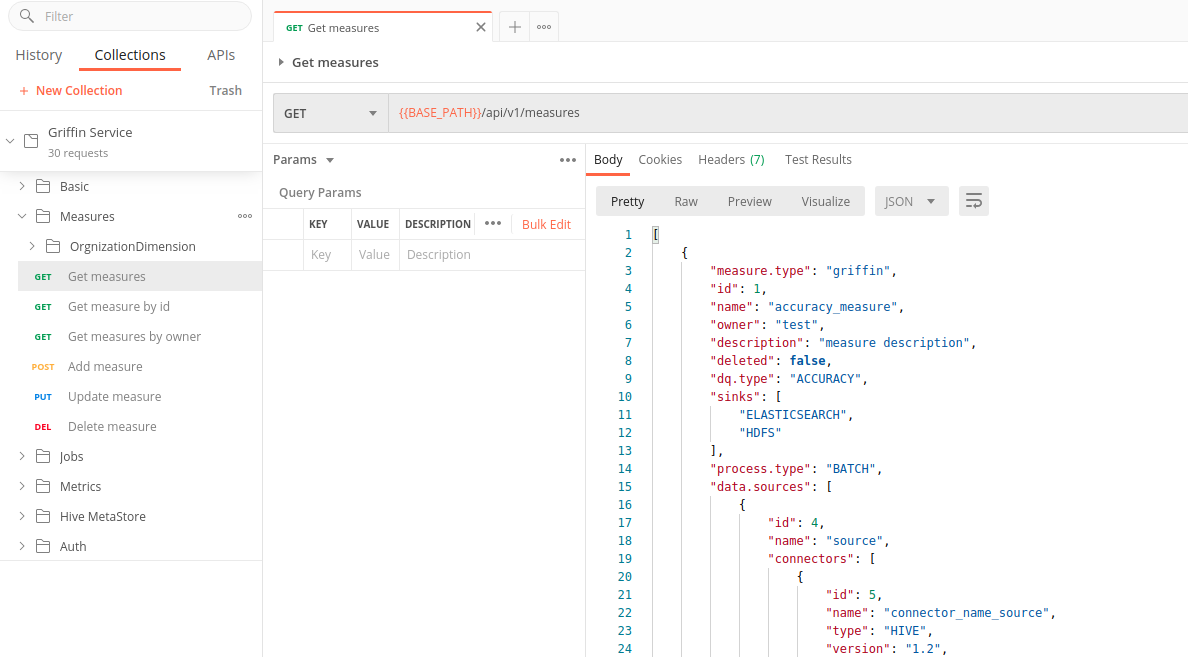
\includegraphics[scale=0.35]{Main/Static/Postman_Griffin.png} 
     \end{center}

\end{figure}
 
%\newpage
\subsubsection{\textbf{Couches de fonctionnement de Apache Griffin}}

Une vue m\'eso de l'architecture de Apache Griffin met en \'evidence trois (3) principales couches: Analyze, Measure et Define chacune jouant un r\^ole fondamental dans le fonctionnement de Griffin. D'abord, nous avons la couche Define, qui est responsable de la d\'efinition des dimensions de qualit\'e. Ensuite, vient la couche Measure qui permet le calcul des diff\'erentes m\'etriques. Les r\'esultats sont stock\'es dans le r\'ef\'erentiel de la derni\`ere couche : Analyze. Elle s'occupe de la sauvegarde et de l'affichage des r\'esultats. 

\begin{figure}[!h]
    \caption{S\'equences de fonctionnement de Apache Griffin}  \label{fig:xray}
    \begin{center}
      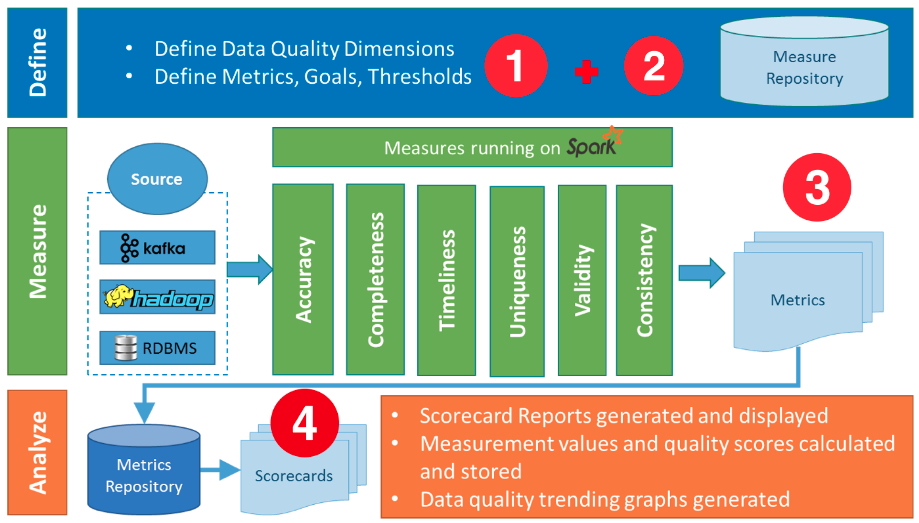
\includegraphics[scale=0.5]{Main/Static/Sequences_de_fonctionnement_Griffin.png} 
    \end{center}
\end{figure}
Suivant cette architecture, on a un flux de travail se pr\'esentant comme suit :

\begin{enumerate}[parsep=0cm,itemsep=0cm]
\item Enregistrement de la source ou des sources de données ;
\item Configuration des r\`egles de qualit\'e, qui peuvent être définies à partir des dimensions de qualité de données ;
\item Planification  de la tâche à soumettre p\'eriodiquement au \textit{cluster} Spark et stockages des m\'etriques;
\item Visualisation des indicateurs sur l'interface et analyser le rendu : la carte thermique et le tableau de bord peuvent \^etre utilis\'es \`a cet effet.

\end{enumerate}
\vspace{0.2cm} 

\subsubsection{\textbf{Infrastructures de l'écosystème d'Apache Griffin}}
Au niveau micro, Apache Griffin est un outil qui d\'epend et utilise plusieurs autres infrastructures \textit{big data} pour l'ex\'ecution des t\^aches. Nul besoin de pr\'eciser qu'on ne saurait parler d'infrastructures \textit{big data} sans citer Apache Hadoop et Apache Spark en premier lieu. Ainsi on y trouve les applications suivantes :

\begin{itemize}[parsep=0cm,itemsep=0cm]
\item \textbf{Apache Hadoop} (version 2.6.0 ou plus) : c'est un \textit{framework} de stockage et de traitement distribu\'e de grands ensembles de donn\'ees sur des \textit{clusters} d'ordinateur. Il sert de source de donn\'ees et au stockage des m\'etriques pour les traitements \textit{batch}. Toute l'architecture repose sur Hadoop;

\item \textbf{Apache Spark }(version 2.2.1 ou plus ): c'est un moteur de calcul distribu\'e et de traitement rapide des donn\'ees, d\'edi\'e au \textit{big data}. Le calcul des m\'etriques est effectu\'e sur Spark pour un gain maximal de performance ;

\item \textbf{Apache Hive} (version 2.x ): il s'agit d'un entrep\^ot de donn\'ees qui sert de \textit{metastore} et \'egalement de source de donn\'ees pour Griffin;

\item \textbf{PostgreSQL} (version 10.4 ou plus) ou \textbf{MySQL} (version 8.0.11 ou plus) :  ce sont des Syst\`emes de Gestion de Bases de Donn\'ees Relationnelles qui servent ici au stockage des diff\'erentes configurations en termes de dimensions de qualit\'e  et ainsi que les d\'etails concernant l'ex\'ecution (model store, asset store, job store) ;

\item \textbf{Livy} : permet de soumettre de façon programmatique des jobs spark  depuis des applications web/mobiles. Il s'agit d'une \acrshort{api} \acrshort{rest}ful ;

\item \textbf{Elasticsearch} (version 5.0 ou plus ): quant \`a lui permet \'egalement de stocker les r\'esultats (m\'etriques) issus de l'analyse de la qualit\'e des donn\'ees;

\item \textbf{Kafka} : Kafka est utilisé principalement pour la mise en place de flux de donn\'ees en temps réel.

\end{itemize}
%\vspace{0.15cm}
Griffin int\`egre \'egalement les d\'ependances suivantes : 

\begin{itemize}[parsep=0cm,itemsep=0cm]
\item \textbf{JDK} pour \acrlong{jdk};
\item \textbf{Scala};
\item \textbf{Maven} qui est un outil de  gestion de projet, utilisé pour empaqueter le projet Apache Griffin en fichier \textit{.jar};
\end{itemize}